% ^^^^^^ This is for TeXworks users ^^^^^
% !TEX root = ../main.tex 
% !TEX program = xelatex
% !TEX encoding = utf-8
% vvvvvv This is for TeXworks users vvvvv

% -*-coding: utf-8 -*-


\defaultfont

\BiChapter{绪论}{ Introduction}
% \label{Introduction}
%   \begin{figure}[htbp] % htbp代表图片插入位置的设置
%     \centering %图片居中
%     %添加图片；[]中为可选参数，可以设置图片的宽高；{}中为图片的相对位置
%     
\includegraphics[width = 0.4\textwidth]{golfer}
%     \caption{滤波对比图} % 图片标题
%     \label{pic8} % 图片标签
%     \end{figure}
\BiSection{课题背景及意义}{ The Background and Significance}
\label{Introduction:background}
在海洋强国战略推动下，水下高精度作业需求持续增长，机械臂的性能直接决定作业效能。
当前主流刚性关节型机械臂依靠电机与减速器独立驱动各关节，负载自重比低、
运动惯性大。在水下机器人-机械手系统（UVMS）中，艇体处于漂浮状态，
受水流与波浪干扰产生低频摇荡\ucite{BIAN2025120845}，刚性臂的高惯性会放大基座扰动，
导致末端抖振漂移，定位精度严重下降，精细作业难以开展\ucite{jmse9101131}，
且缺乏柔顺缓冲，碰撞风险高。

绳驱机械臂通过柔性绳索将驱动后置于艇体，实现驱动与结构分离，
使臂体极致轻量化，从物理层面抑制了基座扰动的传递，并具备被动柔顺安全特性\ucite{Yan2022}。
本文针对UVMS漂浮基座下末端定位精度低的难题，设计绳驱水下机械臂，
将驱动单元内置于艇体、多级绳索传动以超轻量臂体；
进而建立含艇体运动的动力学模型，融合视觉反馈与扰动观测器构建主动补偿控制策略，
实现漂浮基座下高精度轨迹跟踪与稳定抓取。该研究有望为水下精细作业提供轻量、
柔顺且本征抗扰动的新型执行机构，对提升深海自主作业能力、
服务海洋强国战略具有重要理论价值和工程前景。

\begin{figure}[H] % htbp代表图片插入位置的设置
  \setlength{\belowcaptionskip}{1pt}
  \centering %图片居中
  %添加图片；[]中为可选参数，可以设置图片的宽高；{}中为图片的相对位置
  
\includegraphics[width = 0.6\textwidth]{处理图片(1)}
  
  \caption{UVMS示意图} % 图片标题
  \vspace{-0.5cm}
   % 临时修改当前图的下间距
  \label{pic111} % 图片标签
  \end{figure}


% \begin{figure}[H]
%   \centering
%   % 第一张子图
%   \begin{minipage}{0.3\textwidth}
%       \centering
%       \subfigure[ABB IRB2600焊接机械臂]{\label{fig:sub1}
%           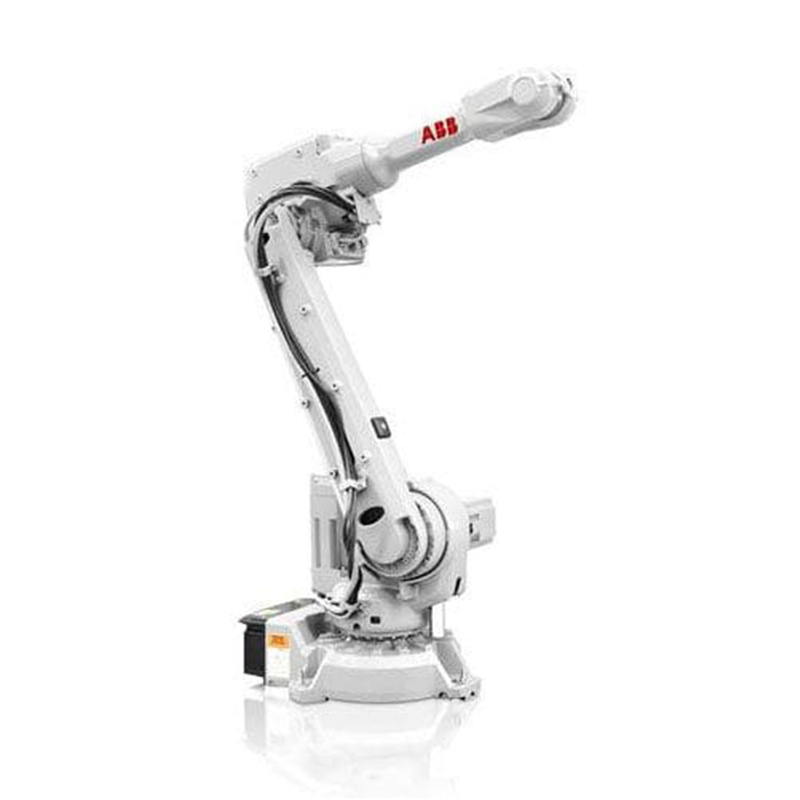
\includegraphics[width = \textwidth]{figures/ABBarm.jpg}
%       }% 这里写第一张图的英文描述
%   \end{minipage}
%   % \hfill % 撑开左右间距
%   % 第二张子图
%   \begin{minipage}{0.45\textwidth}
%       \centering
%       \subfigure[“Super Dragon”绳驱机械臂]{\label{fig:sub2}
%           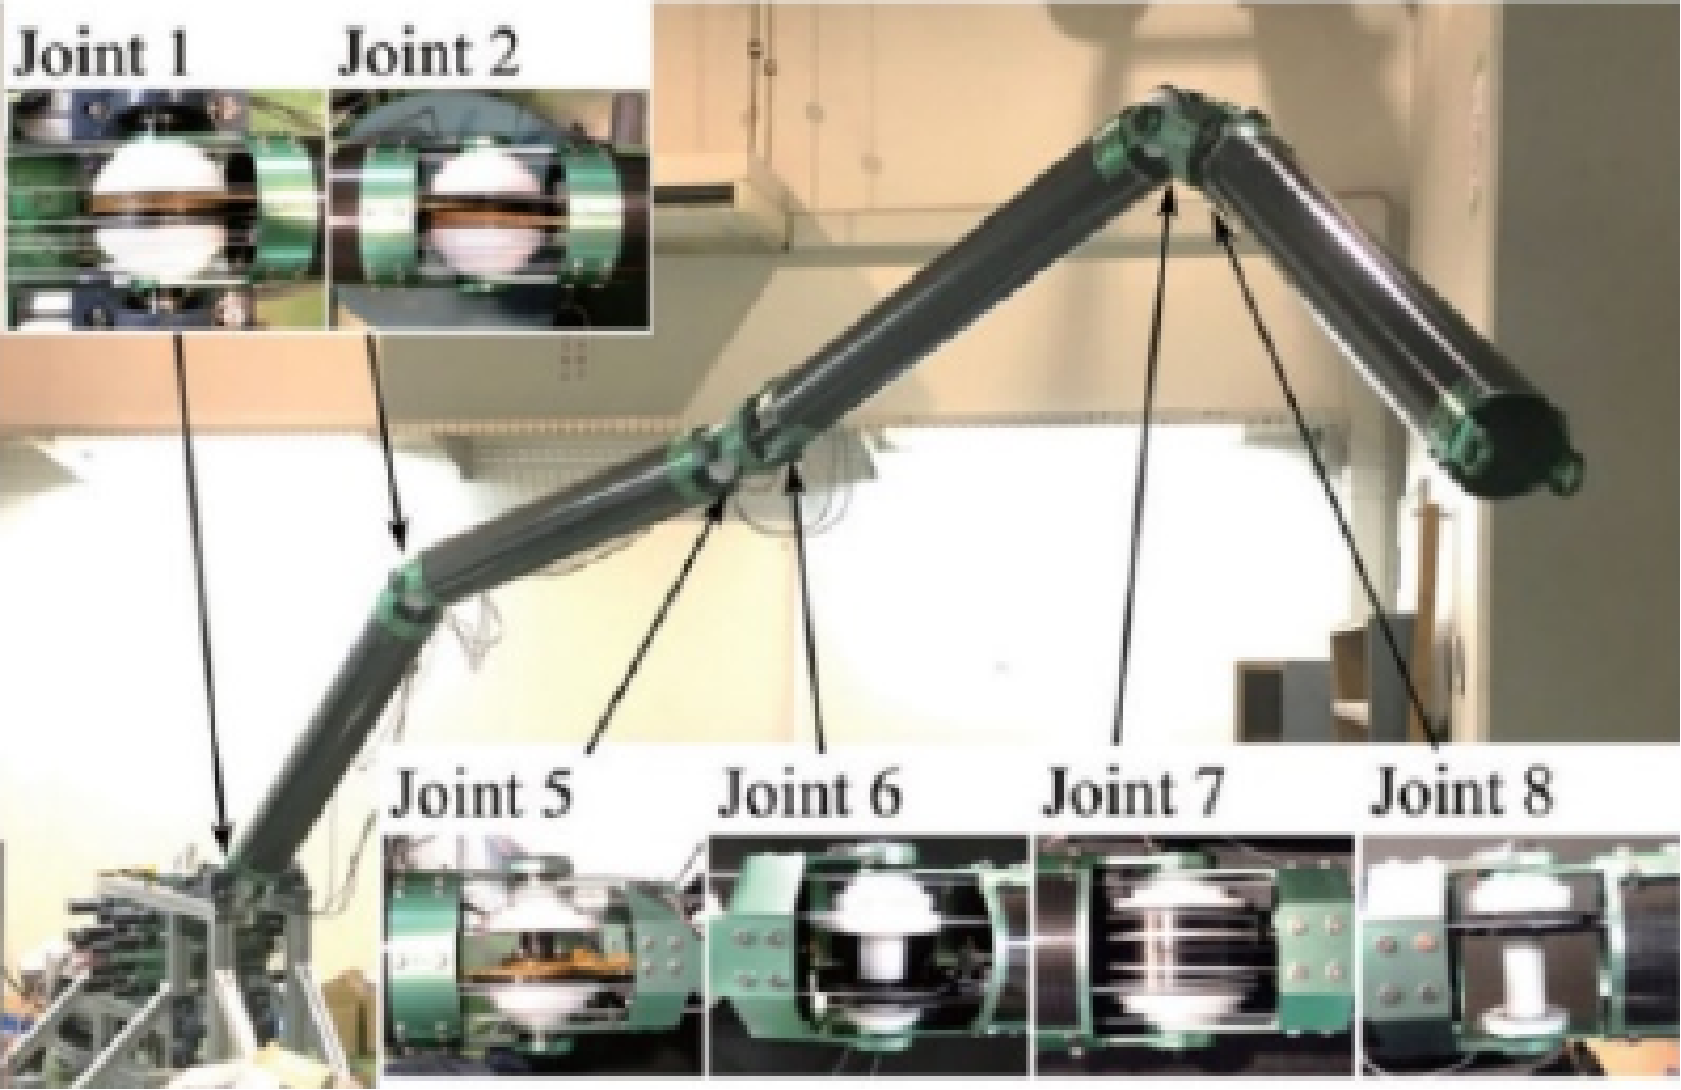
\includegraphics[width = \textwidth]{figures/绳驱机械臂.png}
%       } % 这里写第二张图的英文描述
%   \end{minipage}

%   % 中英文总标题
%   \caption{两类机械臂}
%   \label{fig:total_figure}
% \end{figure}
% \begin{figure}[H]
%   \centering
%   % 第一张子图
%   \begin{minipage}{0.45\textwidth}
%       \centering
%       \subfigure[Girona 500]{\label{fig:sub11}
%           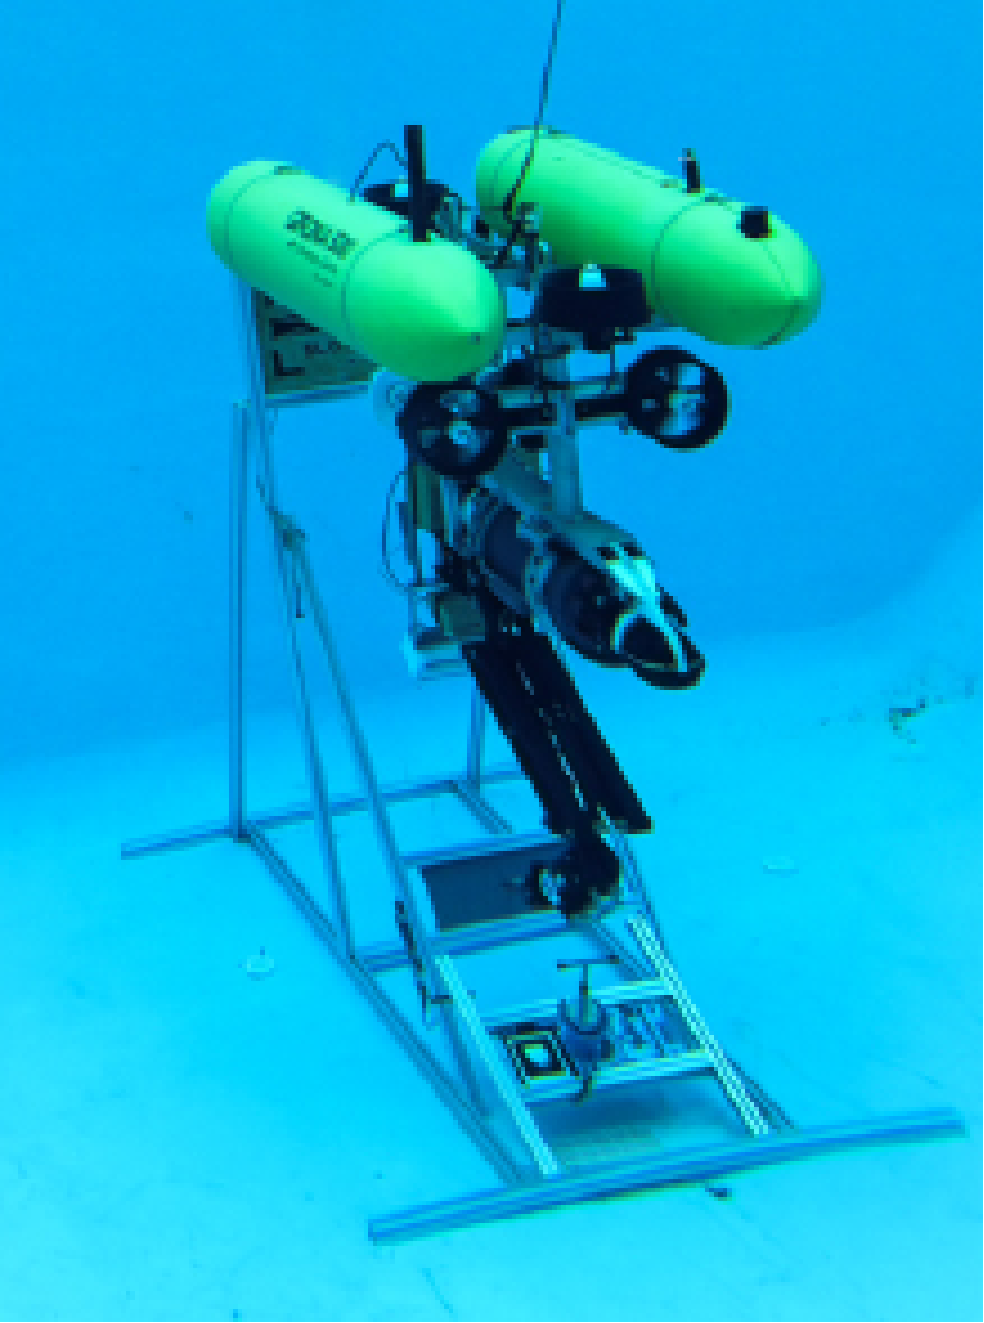
\includegraphics[width = 0.7\textwidth]{figures/rov机械臂系统.png}
%       }
%   \end{minipage}
% %   \hfill % 添加弹性间距，让图片分布均匀
% %   % 第二张子图
% %   \begin{minipage}{0.3\textwidth}
% %       \centering
% %       \subfigure[Twin-Burger]{\label{fig:sub12}
% %           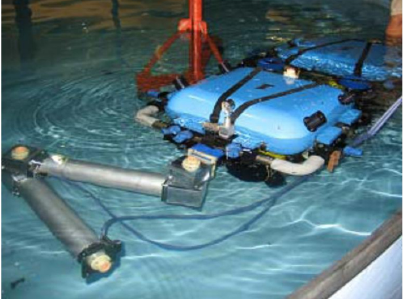
\includegraphics[width = \textwidth]{figures/Snipaste_2026-02-28_13-42-07.png}
% %       }
% %   \end{minipage}
%   \hfill % 添加弹性间距
%   % 第三张子图
%   \begin{minipage}{0.45\textwidth}
%       \centering
%       \subfigure[浙大AUVMS]{\label{fig:sub13}
%           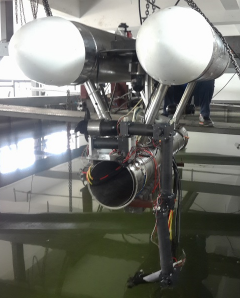
\includegraphics[width = 0.7 \textwidth]{figures/Snipaste_2026-02-28_13-42-13.png}
%       }
%   \end{minipage}
%   % 中英文总标题
%   \caption{AUV-机械臂系统}
%   \label{fig:total_figure1}
% \end{figure}
\BiSection{相关技术国内外研究现状}{Mastering \LaTeX{}}
接下来将针对水下机械臂与绳驱机械臂两种技术进行国内外研究现状进行分析
\BiSubsection{水下机械臂}{Mastering \LaTeX{}}

国外对水下机械臂的研究起步较早，技术成熟度高，
目前已形成从深海重载到核环境特种维护的完整产品体系，
多款设备实现了商业化。

在深海重载作业领域，
美国 Schilling Robotics 公司的 ATLAS 7R 机械臂\ucite{Schilling_ATLAS7R}，
广泛搭载于工作级 ROV。该臂有 6 自由度，作业半径 1.664 m，
自重 73 Kg，最大水下抓取力可达 500Kg。
主体采用高强度钛合金与铝合金，通过液压驱动，
能在 6500 米深海保持较高的作业灵活性。


在核工业特种作业方面，针对高辐射和狭窄空间的需求，
小型化与模块化是一条重要路线。
韩国原子能研究院核机器人技术实验室于 2007 年研制了一款小型水下机械臂，
主要用于反应堆容器底部残余核废料的清理，
如螺栓、螺母和金属碎屑。
该臂采用 5 自由度，展开长度约 60 cm，
具备水下 30 米密封能力，可搭载于微型水下避障平台，
在强辐射环境中替代人工完成高危清理任务。
\begin{figure}[H]
  \centering
  \begin{minipage}{0.4\textwidth}
      \centering
      
\includegraphics[width=0.8\linewidth]{ATALAS7R水下机械臂}
      \caption{ATLAS 7R 水下机械臂}
      \vspace{-0.5cm}
      \label{pic81}
  \end{minipage}
  \hfill
  \begin{minipage}{0.5\textwidth}
      \centering
      
\includegraphics[width=0.8\linewidth]{韩国原子能研究院核机械臂}
      \caption{韩国原子能研究院核机械臂}
      \vspace{-0.5cm}
      \label{pic91}
  \end{minipage}
\end{figure}
1985 年，我国中科院研究所自主研制的首款水下机械臂“海人一号”\ucite{Jiang_HR01_1988}成功下水实验，
如图所示，这款有缆式水下机械臂可以在水深 200 米处进行工作。
配备的水下机械臂使用主从控制模式，能够实现位置与力的双向反馈调节，
从而提升操作的精度与稳定性。这是我国首款完全自主研发的水下机械臂，
标志着该领域的重要技术突破，标志着我国水下机械臂技术发展的起点。

此外，上海交通大学研发的“海龙号”水下机器人在任务执行过程中同样表现
出良好的作业能力。
如图所示，该系统配备有两种类型的水下机械臂分别为七自由度和五自由度结构，
具备远程控制能力，能够在水面指令下完成样品抓取、海底勘探等多种水下作业任务，
展示了其良好的实用性与灵活性。
\begin{figure}[H]
  \centering
  \begin{minipage}{0.45\textwidth}
      \centering
      
\includegraphics[width=\linewidth]{4271}
      \caption{水下机械臂“海人一号”}
      \vspace{-0.5cm}
      \label{pic83}
  \end{minipage}
  \hfill
  \begin{minipage}{0.45\textwidth}
      \centering
      
\includegraphics[width=0.8\linewidth]{4272}
      \caption{“海龙号”水下机器人}
      \vspace{-0.5cm}
      \label{pic93}
  \end{minipage}
\end{figure}
\BiSubsection{绳驱机械臂}{Mastering \LaTeX{}}



在多自由度移动作业系统方面，上海交通大学研制了专门用于物流系统的绳驱动多自由度移动机器人。该研究利用绳索传动的高动态响应特性，解决了传统物流机器人在复杂路径下运动惯性大、能效比低的问题，为大规模自动化仓储环境下的快速作业提供了新的技术思路。
  % \begin{figure}[H] % htbp代表图片插入位置的设置
  %   \centering %图片居中
  %   %添加图片；[]中为可选参数，可以设置图片的宽高；{}中为图片的相对位置
  %   
\includegraphics[width = 0.5\textwidth]{上交机械臂}
  %   \caption{上海交通大学绳驱动多自由度移动机器人} % 图片标题
  %   \label{pic10} % 图片标签
  %   \end{figure}
在高负载轻量化机械臂方面，南京航空航天大学设计并研制了一款7自由度绳驱动机械臂。
该机械臂自身质量为5.8Kg左右，但在末端可实现4Kg的负载能力
，优于传统的电机直驱机械臂。
针对绳索传动中普遍存在的摩擦损耗问题，
该团队采用了滑轮导向的传动方案。
减少了摩擦阻力，提升了机械臂的效率。
  

\begin{figure}[H]
  \centering
  \begin{minipage}{0.45\textwidth}
      \centering
      
\includegraphics[width=0.8\linewidth]{上交机械臂}
      \caption{上海交通大学绳驱机械臂}
      \vspace{-0.5cm}
      \label{pic82}
  \end{minipage}
  \hfill
  \begin{minipage}{0.45\textwidth}
      \centering
      
\includegraphics[width=0.7\linewidth]{南航绳驱机械臂}
      \caption{南航绳驱机械臂}
      \vspace{-0.5cm}
      \label{pic92}
  \end{minipage}
\end{figure}

东京工业大学远藤玄团队针对福岛核电站退役需求研制了 Super Dragon 超长尺耦合腱绳驱动机械臂\ucite{Endo2019SuperDA}。
该臂采用耦合钢丝绳传动与合成纤维绳索重力补偿，驱动单元全部后置，
使原型机在总长 10 m、最大臂径仅 0.2 m、配置 10 个关节的条件下实现轻量化。
团队提出基于双滑轮的机械式增稳方法，抑制了长距绳索传动的不稳定行为，
并将臂长进一步拓展至 15.4 m；同时利用拮抗张力控制将工作域体积扩大了 45\%。

清华大学设计了一款6自由度全解耦绳驱动机械臂\ucite{Chen2011}。重量仅为1.6Kg，
具有1.29毫米的平均定位误差和2.0公斤的负载能力。
采用滚动关节，成功解耦了肘部运动和腕部肌腱的运动。
此外，通过每个关节处的长度补偿器实现了全关节解耦。

\begin{figure}[H]
  \centering
  \begin{minipage}{0.45\textwidth}
      \centering
      
\includegraphics[width=1.0\linewidth]{东京}
      \caption{“Super Dragon”机械臂}
      \vspace{-0.5cm}
      \label{pic84}
  \end{minipage}
  \hfill
  \begin{minipage}{0.45\textwidth}
      \centering
      
\includegraphics[width=0.8\linewidth]{清华}
      \caption{清华全解耦绳驱机械臂}
      \vspace{-0.5cm}
      \label{pic92}
  \end{minipage}
\end{figure}

\BiSection{论文主要工作内容}{Main Research Contents}

本文围绕水下绳驱机械臂的结构设计、运动学建模、视觉抓取与试验样机搭建开展研究。主要工作内容及章节安排如下：

% 第一章 绪论：阐述水下运载器、水下机械臂及绳驱技术的研究背景与意义，分析国内外的研究现状，提出本文的研究目标与主要工作内容。
    
第二章进行水下绳驱机械臂结构研制。根据水下小型运载器的需求，提出将驱动元件后置于独立密封舱的绳驱方案。完成水平旋转肩关节、肘部双铰链滚动关节及腕关节的机械结构设计；设计全滑轮导向的驱动绳走线及自锁张紧机构；完成驱动舱的动/静密封设计，并对大臂、滑轮轴等关键部件进行理论力学计算与 ANSYS 有限元静力学仿真校核。
    
第三章对水下绳驱机械臂进行运动学建模。基于改进 D-H 法建立机械臂的正运动学模型；采用牛顿-拉夫逊数值迭代法进行逆运动学求解，并推导了驱动空间与关节空间的耦合关系。在此基础，分别在关节空间进行了多项式与梯形速度轨迹规划，在笛卡尔空间实现直线与圆弧轨迹的插补，并通过 MATLAB 仿真验证算法的有效性。

第四章研究单目视觉的目标定位与抓取策略研究。针对自主抓取，建立单目相机模型并完成相机内外参标定；采用“眼在手外”构型，基于 ArUco 特征标记物完成手眼标定，构建从二维图像坐标系到机械臂物理坐标系的空间位姿映射，并设计了目标位姿估计与抓取控制上位机程序。
    
第五章 试验样机搭建与试验研究。搭建以“树莓派 + STM32”主从架构为核心的试验平台，开发了基于 ROS 2 分布式架构的控制系统软件平台。开展机械臂基础运动测试、空间轨迹规划验证以及视觉引导下的闭环抓取实验，对机械臂的运动性能及末端定位误差进行分析。
    
% 结论：总结全文的主要研究成果，指出当前研究及样机存在的不足，并对未来水下绳驱机械臂的改进与研究方向进行展望。
\clearpage{
  \pagestyle{plain}
  \cleardoublepage
}
%%% Local Variables: 
%%% mode: latex
%%% TeX-master: "../main"
%%% End: 
